% Undergraduate Project Presentation Template
% Compile with: pdflatex UG_Project_Presentation_Template.tex
% Recommended: Overleaf or TeX Live/MiKTeX with the packages below.

\documentclass[aspectratio=169,11pt]{beamer}

% ---------- Theme and colours ----------
\usetheme{Madrid}
\usecolortheme{default}
\definecolor{UniversityBlue}{RGB}{16,62,110}
\definecolor{AccentBlue}{RGB}{30,136,229}
\definecolor{LightBlue}{RGB}{232,242,252}
\definecolor{DarkGray}{RGB}{55,65,81}

\setbeamercolor{structure}{fg=UniversityBlue}
\setbeamercolor{palette primary}{bg=UniversityBlue,fg=white}
\setbeamercolor{palette secondary}{bg=AccentBlue,fg=white}
\setbeamercolor{frametitle}{bg=UniversityBlue,fg=white}
\setbeamercolor{block title}{bg=UniversityBlue,fg=white}
\setbeamercolor{block body}{bg=LightBlue,fg=black}
\setbeamercolor{alerted text}{fg=AccentBlue}

% ---------- Packages ----------
\usepackage[T1]{fontenc}
\usepackage[utf8]{inputenc}
\usepackage{lmodern}
\usepackage{graphicx}
\usepackage{booktabs}
\usepackage{array}
\usepackage{tabularx}
\usepackage{tikz}
\usetikzlibrary{positioning}
\usepackage{amsmath}
\usepackage{listings}
\usepackage{xcolor}
\usepackage{colortbl}
\usepackage{hyperref}

% ---------- General settings ----------
\setbeamertemplate{navigation symbols}{}
\setbeamertemplate{caption}[numbered]
\setbeamertemplate{itemize item}{\color{AccentBlue}$\blacktriangleright$}
\setbeamertemplate{itemize subitem}{\color{UniversityBlue}$\bullet$}
\setbeamersize{text margin left=0.7cm,text margin right=0.7cm}

% Footer: project title, institution and slide number
\setbeamertemplate{footline}{%
  \leavevmode%
  \hbox{%
    \begin{beamercolorbox}[wd=.42\paperwidth,ht=2.7ex,dp=1.1ex,leftskip=.6em]{author in head/foot}%
      \insertshorttitle
    \end{beamercolorbox}%
    \begin{beamercolorbox}[wd=.46\paperwidth,ht=2.7ex,dp=1.1ex,center]{date in head/foot}%
      Department of Computer Science and Engineering
    \end{beamercolorbox}%
    \begin{beamercolorbox}[wd=.12\paperwidth,ht=2.7ex,dp=1.1ex,center]{page number in head/foot}%
      \insertframenumber/\inserttotalframenumber
    \end{beamercolorbox}%
  }%
  \vskip0pt%
}

% ---------- Code style ----------
\lstset{
  basicstyle=\ttfamily\scriptsize,
  keywordstyle=\color{UniversityBlue}\bfseries,
  commentstyle=\color{gray},
  stringstyle=\color{AccentBlue},
  numbers=left,
  numberstyle=\tiny\color{gray},
  frame=single,
  breaklines=true,
  showstringspaces=false
}

% ---------- Editable project details ----------
\title[Short Project Title]{Your Undergraduate Project Title}
\subtitle{Initial / Zeroth / Phase-I / Second Review / Final Review}
\author[Student Team]{%
  Student Name 1 (Register No.)\\
  Student Name 2 (Register No.)\\
  Student Name 3 (Register No.)
}
\institute[University Name]{%
  Guided by: Dr. Guide Name, Designation\\[2mm]
  Department of Computer Science and Engineering\\
  College / University Name
}
\date{Academic Year 2026--2027}

\begin{document}

% 1. Title slide
\begin{frame}[plain]
  \titlepage
  % Optional logo:
  % \begin{tikzpicture}[remember picture,overlay]
  %   \node[anchor=north east,xshift=-0.4cm,yshift=-0.3cm]
  %   at (current page.north east){\includegraphics[width=1.5cm]{college-logo.png}};
  % \end{tikzpicture}
\end{frame}

% First Review Queries - Answers
\begin{frame}{First Review - Queries and Answers}
      Answer the Queries raised in First Review
\end{frame}

%\section{Introduction}
% 4. Problem statement
\begin{frame}{Problem Statement}
  \begin{alertblock}{Problem}
    Existing systems face \textbf{[specific limitation]}, resulting in
    \textbf{[measurable impact]} for \textbf{[target users/stakeholders]}.
  \end{alertblock}
  \vspace{0.4cm}
  \begin{itemize}
    \item What is the exact technical or societal problem?
    \item What causes the problem?
    \item Why are existing approaches insufficient?
    \item What constraints must the solution satisfy?
  \end{itemize}
\end{frame}

% 5. Objectives
\begin{frame}{Project Objectives}
  \begin{enumerate}
    \item To analyse \textbf{[domain/problem]} and identify its key requirements.
    \item To design a \textbf{[system/model/framework]} for \textbf{[purpose]}.
    \item To implement the proposed solution using \textbf{[tools/technologies]}.
    \item To evaluate the solution using \textbf{[metrics/test criteria]}.
    \item To compare the proposed solution with \textbf{[baseline/existing system]}.
  \end{enumerate}
\end{frame}

%\section{System Design}
% 10. Architecture
\begin{frame}{Proposed System Architecture}
  \centering
  % Preferred: export the architecture diagram as PDF/PNG and insert it here.
  % \includegraphics[width=0.88\textwidth,height=0.68\textheight,keepaspectratio]{architecture.pdf}
  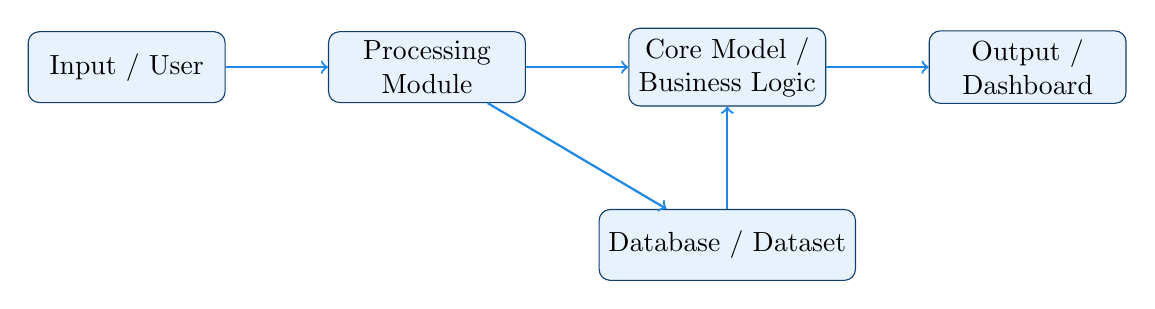
\begin{tikzpicture}[node distance=1.3cm,
      box/.style={draw=UniversityBlue,fill=LightBlue,rounded corners,
                  minimum width=2.5cm,minimum height=0.9cm,align=center},
      arrow/.style={->,thick,draw=AccentBlue}]
    \node[box] (input) {Input / User};
    \node[box,right=of input] (process) {Processing\\Module};
    \node[box,right=of process] (model) {Core Model /\\Business Logic};
    \node[box,right=of model] (output) {Output /\\Dashboard};
    \draw[arrow] (input) -- (process);
    \draw[arrow] (process) -- (model);
    \draw[arrow] (model) -- (output);
    \node[box,below=of model] (data) {Database / Dataset};
    \draw[arrow] (process) -- (data);
    \draw[arrow] (data) -- (model);
  \end{tikzpicture}
  \vspace{0.5cm}

  \small Replace the sample with the actual architecture and explain the data flow.
\end{frame}

% 11. Modules
\begin{frame}{System Modules}
  \begin{enumerate}
    \item \textbf{Module 1 -- Data/Input Management:} Brief purpose and inputs.
    \item \textbf{Module 2 -- Preprocessing:} Cleaning, validation, or transformation.
    \item \textbf{Module 3 -- Core Processing:} Algorithm, model, or business logic.
    \item \textbf{Module 4 -- Storage/API:} Data persistence and service interfaces.
    \item \textbf{Module 5 -- User Interface:} Outputs, reports, and interactions.
  \end{enumerate}
\end{frame}

% 12. Methodology
\begin{frame}{Methodology / Workflow}
  \begin{columns}[T,onlytextwidth]
    \column{0.62\textwidth}
      \begin{enumerate}
        \item Requirement analysis and data collection
        \item Data preparation / system design
        \item Model or algorithm development
        \item Application integration
        \item Testing and performance evaluation
        \item Deployment and documentation
      \end{enumerate}
    \column{0.34\textwidth}
      \begin{block}{Evaluation Metrics}
        \begin{itemize}
          \item Accuracy / F1-score
          \item Response time
          \item Resource usage
          \item User satisfaction
        \end{itemize}
      \end{block}
  \end{columns}
\end{frame}

% 13. Algorithm
\begin{frame}{Core Algorithm / Processing Logic}
  \begin{block}{Algorithm: [Insert Algorithm Name]}
    \begin{enumerate}
      \item Receive and validate the input $X$.
      \item Transform $X$ into the required representation $X'$.
      \item Apply the proposed method $f(\cdot)$ to obtain $Y=f(X')$.
      \item Evaluate $Y$ using the selected metric(s).
      \item Return or display the final result.
    \end{enumerate}
  \end{block}
  \vspace{0.2cm}
  \small Include equations, pseudocode, or a flowchart only when it improves clarity.
\end{frame}

%\section{Implementation and Results}

% 15. Implementation status
\begin{frame}{Implementation Status}
  \small
  \begin{tabularx}{\textwidth}{X>{\centering\arraybackslash}p{2.2cm}X}
    \toprule
    \textbf{Modules} & \textbf{Status} & \textbf{Evidence / Remarks} \\
    \midrule
    Module 1 & Completed & Pseducode - Executed  \\
    Module 2 & In progress & Mention completed functions  \\
    Module 3 & In progress & Mention completed functions \\
    Module 4 & Planned & Target completion date \\
    \bottomrule
  \end{tabularx}
\end{frame}

% 16. Screenshots
\begin{frame}{Prototype / Implementation Screenshots}
  \begin{columns}[T,onlytextwidth]
    \column{0.48\textwidth}
      \centering
      \fbox{\parbox[c][4.1cm][c]{0.92\linewidth}{\centering Insert Screenshot 1}}

      \small Login / Input / Main Screen
    \column{0.48\textwidth}
      \centering
      \fbox{\parbox[c][4.1cm][c]{0.92\linewidth}{\centering Insert Screenshot 2}}

      \small Output / Dashboard / Result Screen
  \end{columns}
\end{frame}

% 17. Results
\begin{frame}{Results and Performance Analysis}
  \begin{columns}[T,onlytextwidth]
    \column{0.53\textwidth}
      \centering
      % Replace with an exported chart image or pgfplots chart.
      \fbox{\parbox[c][4.3cm][c]{0.92\linewidth}{\centering Insert Result Chart / Confusion Matrix}}
    \column{0.43\textwidth}
      \begin{block}{Key Findings}
        \begin{itemize}
          \item Metric 1: \textbf{XX.XX\%}
          \item Metric 2: \textbf{X.XX}
          \item Improvement: \textbf{XX\%}
          \item Main observation from testing
        \end{itemize}
      \end{block}
  \end{columns}
\end{frame}

%\section{Project Management}
% 20. Responsibilities
\begin{frame}{Team Responsibilities}
  \small
  \begin{tabularx}{\textwidth}{>{\bfseries}p{3.3cm}X p{2.3cm}}
    \toprule
    Team Member & Responsibilities & Current Status \\
    \midrule
    Student 1 & Literature review, module design, documentation & In progress \\
    Student 2 & Data preparation, backend/model implementation & In progress \\
    Student 3 & Frontend, integration, testing and deployment & In progress \\
    \bottomrule
  \end{tabularx}
\end{frame}

%\section{Conclusion}
% 23. References
\begin{frame}[allowframebreaks]{References}
  \footnotesize
  \begin{thebibliography}{9}
    \bibitem{ref1}
      A. Author and B. Author,
      ``Title of the journal/conference paper,''
      \emph{Journal or Conference Name}, vol. X, no. Y, pp. 1--10, 2025.

    \bibitem{ref2}
      C. Author,
      \emph{Title of the Book}.
      Publisher, 2024.

    \bibitem{ref3}
      Organisation Name,
      ``Title of dataset, standard, or web resource,'' 2026.
      [Online]. Available: \url{https://example.org}
  \end{thebibliography}
\end{frame}

% 24. Thank you
\begin{frame}[plain]
  \centering
  \vfill
  {\usebeamerfont{title}\color{UniversityBlue}\Huge Thank You}\par
  \vspace{0.5cm}
  {\Large Questions and Discussion}\par
  \vspace{0.8cm}
  \vfill
\end{frame}

\end{document}
